\documentclass{article}

\usepackage[margin=1in]{geometry}
\usepackage{amsmath}
\usepackage{float}
\usepackage{amsfonts}
\usepackage{graphicx}

\author{\begin{tabular}{l@{\hspace{2em}}r}Zachary \textsc{Vogel}& Maurice \textsc{Woods} III\end{tabular}\\[1.5ex]
\begin{tabular}{l@{\hspace{1.5em}}r}Derek \textsc{Reamon} & Mechatronics\end{tabular}
}
\date{\today}
\title{\textbf{\begin{tabular}{c}Grad Project Equations in MCEN 5115:\\Rotating Inverted Pendulum\end{tabular}}}

\begin{document}
\maketitle

\section*{Normal Inverted Pendulum}
\begin{figure}[H]
    \centering
    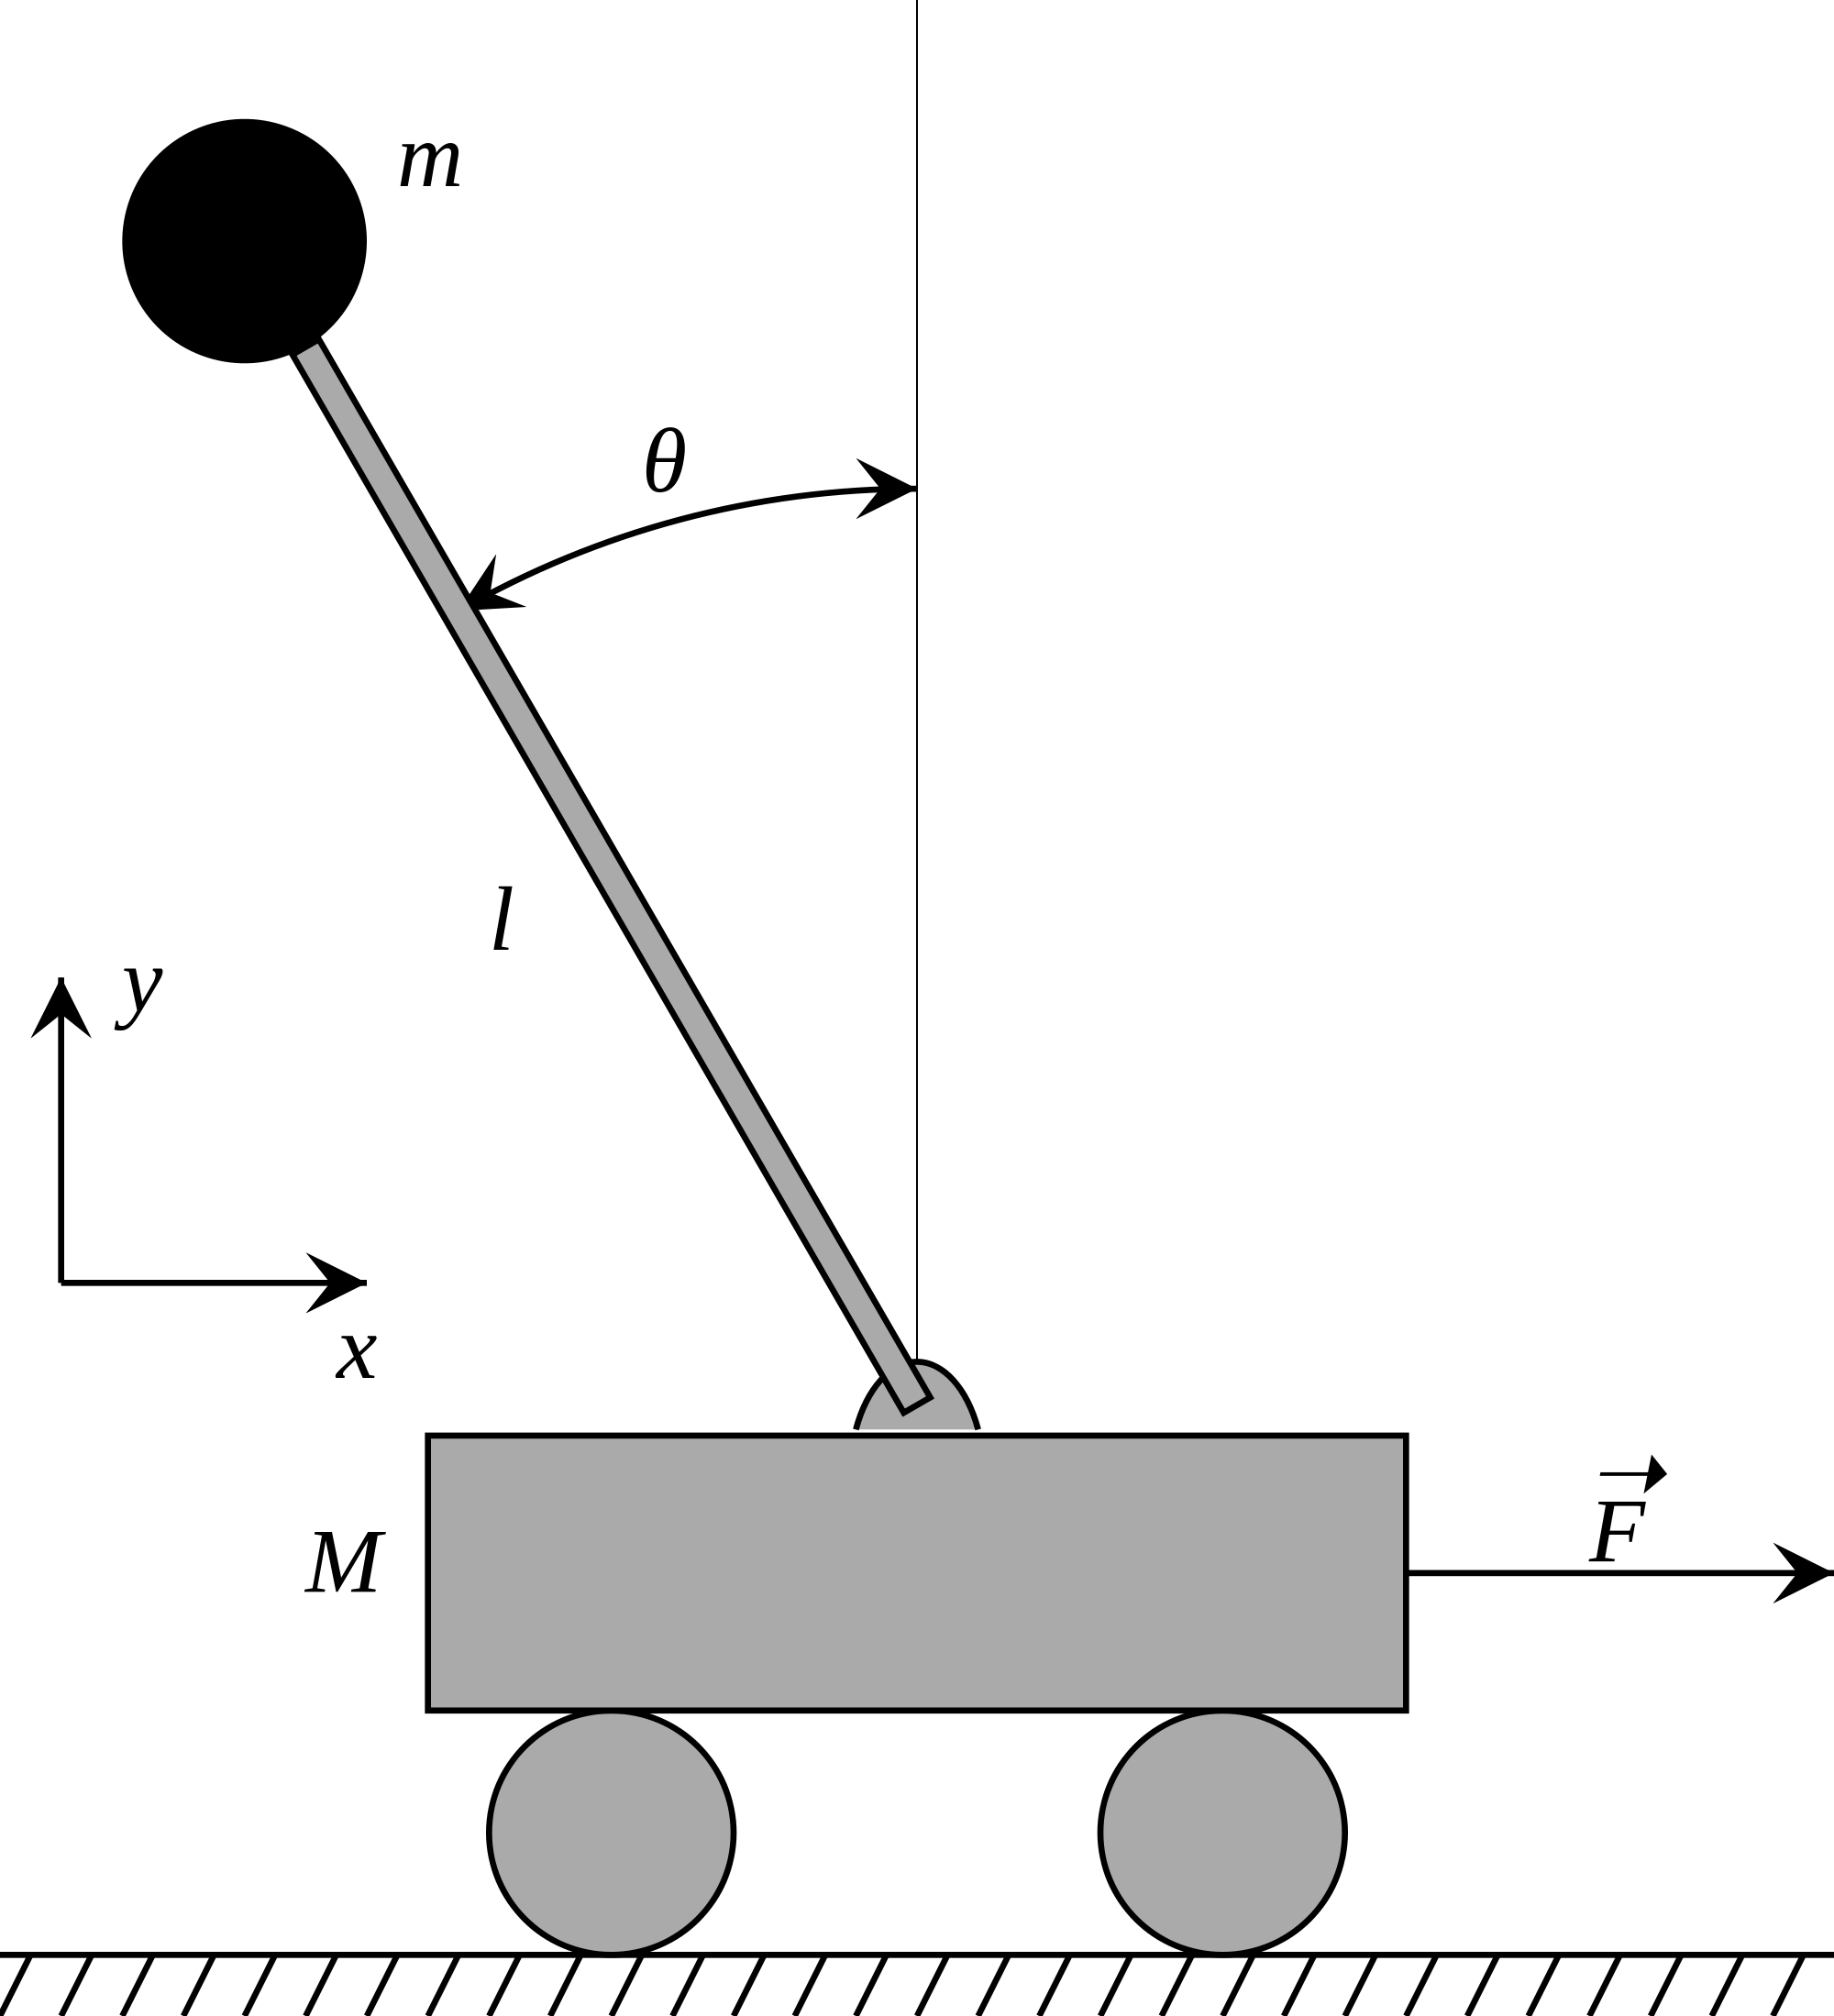
\includegraphics[width=0.7\textwidth]{inv_pend.png}
    \caption{sup sup}
\end{figure}
Here we have the normal inverted pendulum equations for the image above:
\[\begin{split}(M+m)\ddot{x}-ml\ddot{\theta}+ml(\dot{\theta})^2\sin(\theta)=F\\l\ddot{\theta}-g\sin(\theta)=\ddot{x}\cos(\theta)\end{split}\]
The $x$ position for us is actually $\omega$ because we are spinning. Also, the input force isn't $F$. What we have is a torque $\tau=\lvert\lvert r\rvert\rvert\lvert\lvert F\rvert\rvert\sin(\theta)$. Given that the $\theta$ here is 90 degrees or 270 degrees, force can be equated to $F=\frac{\tau}{r}$.\\
Torque is some function of the motor current and the motor properties that we can put in later. We also note that $x=\omega*r$ and thus $\ddot{x}=\ddot{\omega}r$.\\
Thus our equations become:
\[\begin{split}\cfrac{\tau}{r}=ml(\dot{\theta})^2\sin(\theta)-ml\ddot{\theta}+(M+m)\ddot{\omega}r\\\ddot{\omega}r\cos(\theta)=l\ddot{\theta}-g\sin(\theta)\end{split}\]



\end{document}
